To record a demonstration, here is the process: the robot starts somewhere while executing a behavior, user provides a correction interactively, the robot reaches the at tractor and must isolate the correction applied in the demonstration data.


\subsection{Algorithm}

When recording a demonstration, the robot is sending data. The data is composed by many different types such as the position points of the robot, the velocity or the force applied for each of those points. This data represents the complete demonstration, it will be an input for the correction isolation algorithm. This algorithm has to extract the correction by finding the beginning and the end.

\subsubsection{Position and Velocity input}

One way to do is to analyze the angle between the velocity vector and the original trajectory (which is a direction that is returned from the dynamical system from any point in the space to the attractor). If those vectors are not aligned, the point is part of a correction.\\

\begin{figure}[H]
\centering
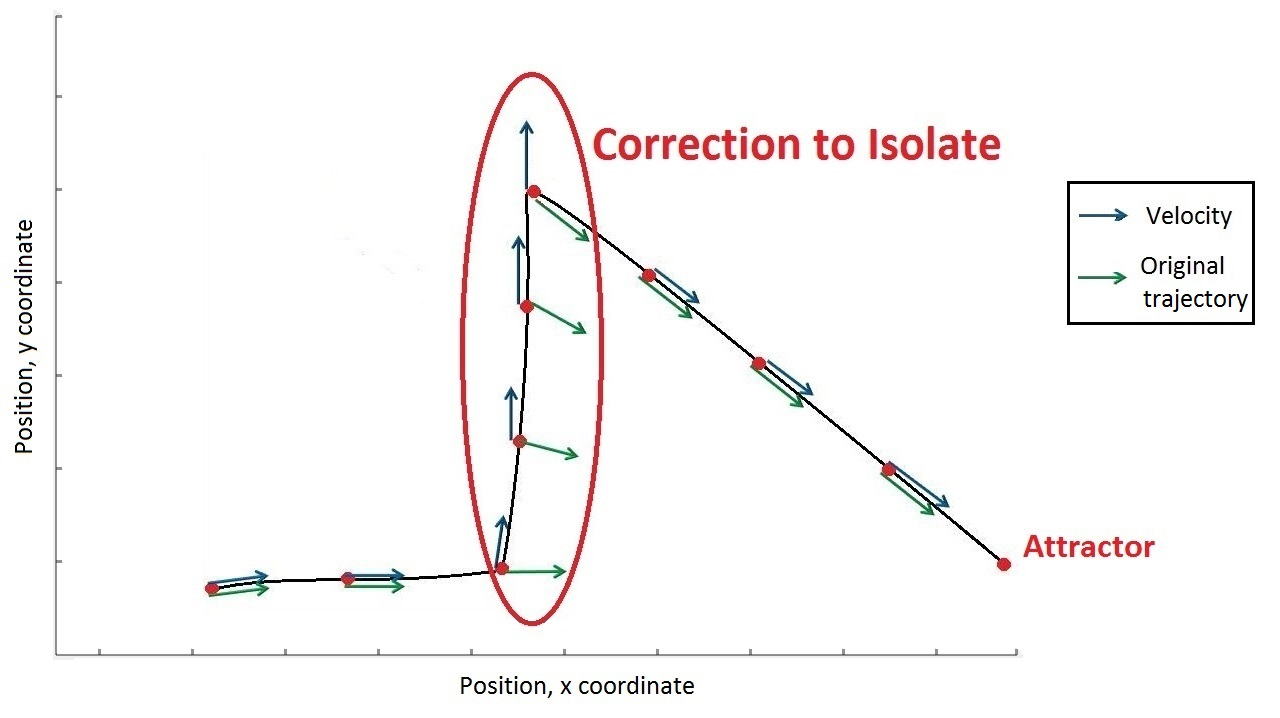
\includegraphics[width=15cm]{img/correction_isolation_1.jpg}
\caption{Demonstration containing one correction.}
\label{correction_isolation_grph}
\end{figure}

As we can see in \autoref{correction_isolation_grph}, when vectors are pointing to a different direction, it means that the point is part of the correction.
To easily find the angle between two vectors, we implement a dot product.

$$ \overrightarrow{Velocity}\ \cdot\ \overrightarrow{Original} = \parallel\overrightarrow{Velocity}\parallel\ \parallel\overrightarrow{Original}\parallel
\cos(\overrightarrow{Velocity},\overrightarrow{Original})$$

Vectors are both normalized, so if they are aligned, the cosine of the angle will be equal to 1.\\

Also, there is always noise in measurement and numerical computations, therefore it wouldn't be appropriate to verify that the vectors are exactly aligned. To do so, a precision factor is added.

\begin{figure}[H]
\centering
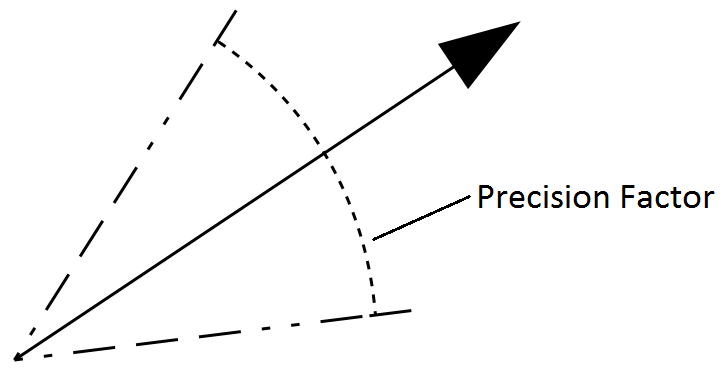
\includegraphics[width=10cm]{img/precision_angle.png}
\caption{Graphical effect of the precision factor on vector comparison.}
\label{graphical_display_factor}
\end{figure}

If the other vector is in the angle interval, then it means that they are considered to be aligned, see \autoref{graphical_display_factor}. The precision factor is implemented as a simple threshold, it makes the algorithm parameterizable see Algorithm \autoref{iso_algo}.
\\
\\
$\vec{v_1}$ and $\vec{v_2}$ are aligned if: $ \cos(\overrightarrow{Velocity}, \overrightarrow{Original}) > 1 - precision factor $
\\
\begin{algorithm}[H]
  \caption{Correction isolation}
  \label{iso_algo}
  \begin{algorithmic}
  \STATE input : demonstration (provide x,y,z,x',y',z' which are the coordinates of each point)
  \STATE

    \FOR{$i\ in\ demonstration$}
      \STATE $dotproduct = x_ix'_i + y_iy'_i + z_iz'_i$

      \IF {$correction\_detected = false$ \AND $dotproduct < (1 - precision\_factor)$}
        \STATE $correction\_detected = true$
        \STATE $beginning\_correction = i$
      \ELSIF{$correction\_detected = true$ \AND $dotproduct > (1 - precision\_factor)$}
        \STATE $correction\_detected = false$
        \STATE $end\_correction = i$
      \ENDIF
    \ENDFOR

  \STATE
  \STATE output : $beginning\_correction$ and $end\_correction$, designate the first and last point of the correction
  \end{algorithmic}
\end{algorithm}

This algorithm could also detect many corrections in a single demonstration by storing many values in $beginning\_correction$ and $end\_correction$, therefore the Boolean variable $correction\_detected$ will switch value many times.

\clearpage

\subsubsection{Force applied input}

The robot also provides information about the external force applied on the arm for each point. Indeed, when an operator applies a correction, he applies a force on the robot with his hand. The aim of this algorithm is to detect this external force. Thus, by computing the norm (to make the algorithm robust for each axis), it's possible to find very precisely the point when a correction starts or ends, see \autoref{force_graph}.

\begin{figure}[H]
\centering
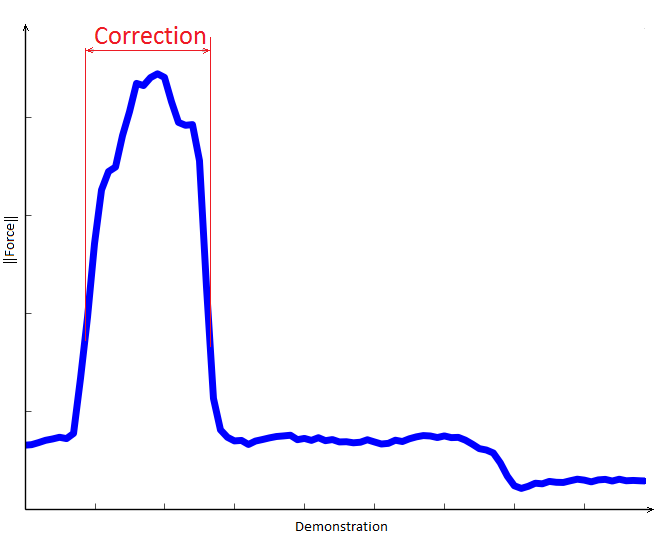
\includegraphics[width=10cm]{img/force_graph.png}
\caption{Graph of the norm of external force applied during a demonstration.}
\label{force_graph}
\end{figure}

The algorithm is exactly the same as Algorithm \autoref{iso_algo}, it's a threshold, when values are going up to a threshold value, it means that they are part of a correction.\\

This algorithm is very precise but is not applicable on any other robot, indeed not all robots measure the applied force. That's why we will consider it as a ground truth for quantitative analysis, but the position and velocity input algorithm will be selected for this application.

\clearpage
\subsection{Algorithm analysis}

To do a quantitative analysis, we made many demonstrations on the robot, and using the force algorithm as a ground truth, we tested the precision factor.\\

Here are the different steps of the analysis: for every demonstration, the force algorithm is applied to find the real correction. The standard velocity algorithm is then applied many times by varying the precision factor from 0 to 1. The result of both algorithms is compared by taking each point that is considered to be in the correction from the velocity, and a percentage of the detected correction is computed with the \autoref{percent_ratio}. Finally, the mean of the percentage of all the curves from all corrections was computed.

\begin{equation}
\label{percent_ratio}
ratio = \frac{Number\ of\ point\ in\ the\ detected\ correction\ and\ also\ in\ the\ real\ correction}{Number\ of\ point\ in\ the\ real\ correction}
\end{equation}

The detected correction is the output of the correction isolation algorithm based on the velocity and the real one is the algorithm based on the force applied on the robot.

\begin{figure}[H]
\centering
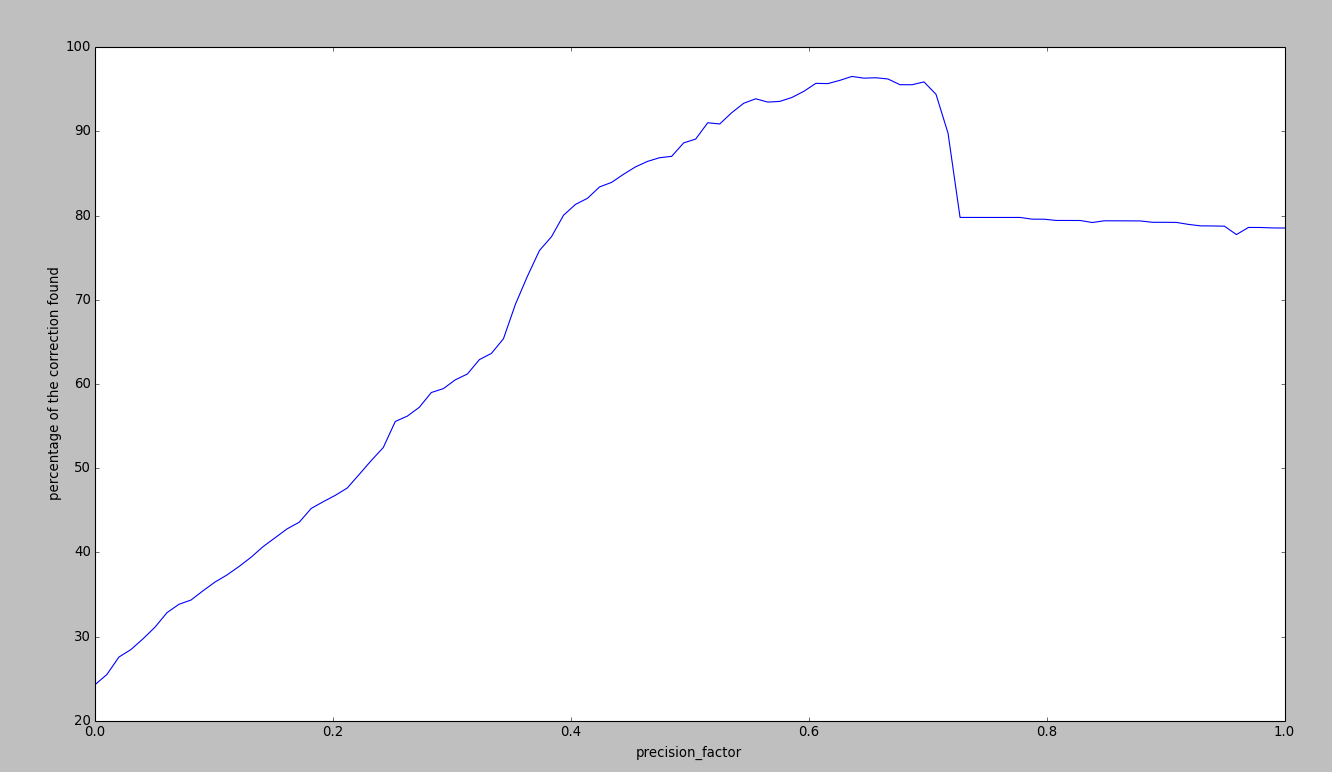
\includegraphics[width=15cm]{img/analysis_algo_iso.png}
\caption{Average of the percentage of the curve detected in terms of the precision factor from 5 demonstrations.}
\label{groundtest_corrections_isolation}
\end{figure}

Based on the few demonstrations correction detection results in \autoref{groundtest_corrections_isolation}, the precision factor seems to give a good result at a value of $\simeq 0.65$.
This result could be used but is absolutely not a reference. \\

With a precision factor of $0.65$, the algorithm will consider that a vector $\vec{v_1}$ is aligned with another vector $\vec{v_2}$ if the cosine is bigger than $0.65$: $cos(\vec{v_1}, \vec{v_2})>0.65$, in other terms, the angle between $\vec{v_1}$ and $\vec{v_2}$ has to be bigger than $49\ degrees$.
